\section{Introduction}
\label{sec:intro}

Consider an OLAP scenario: a database describes how a set of \emph{measures}
varies along several \emph{dimensions}.  To work with this database, analysts
need prior knowledge. To gain this knowledge, they need to \emph{explore}
their data.  During this phase, they try to understand how the
measures are distributed, and why. \emph{How can we suggest queries to
these explorers?} 

We believe that query recommendation is essential to make data analysts more
productive. Informations which are trivial for domain experts are not
necessairily so for data specialists. Besides, experts themselves may need
guidance. Consider for instance Figure \ref{intro}. The table shows a small
extract from a dataset of astronomical observations\footnote{This dataset come
from the LOFAR research programme, 21 May 2012, the Netherlands}. This set
describes the \emph{luminosity} of more than 100,000 sources, taken at
different times, frequency ranges and with different precisions. In total,
there are more than fifty dimensions. Even for an astronomer, this dataset
cannot be understood by intuition alone. We need intelligent navigation tools
to provide guidance.  The bottom picture illustrates what
we expect from our query recommendation tool: a simpler low dimension view, which reveals
particularly bright or large sources. Thanks to this view, anyone can 
quickly perceive interesting regions in the database.

\begin{figure}[t!]
\centering
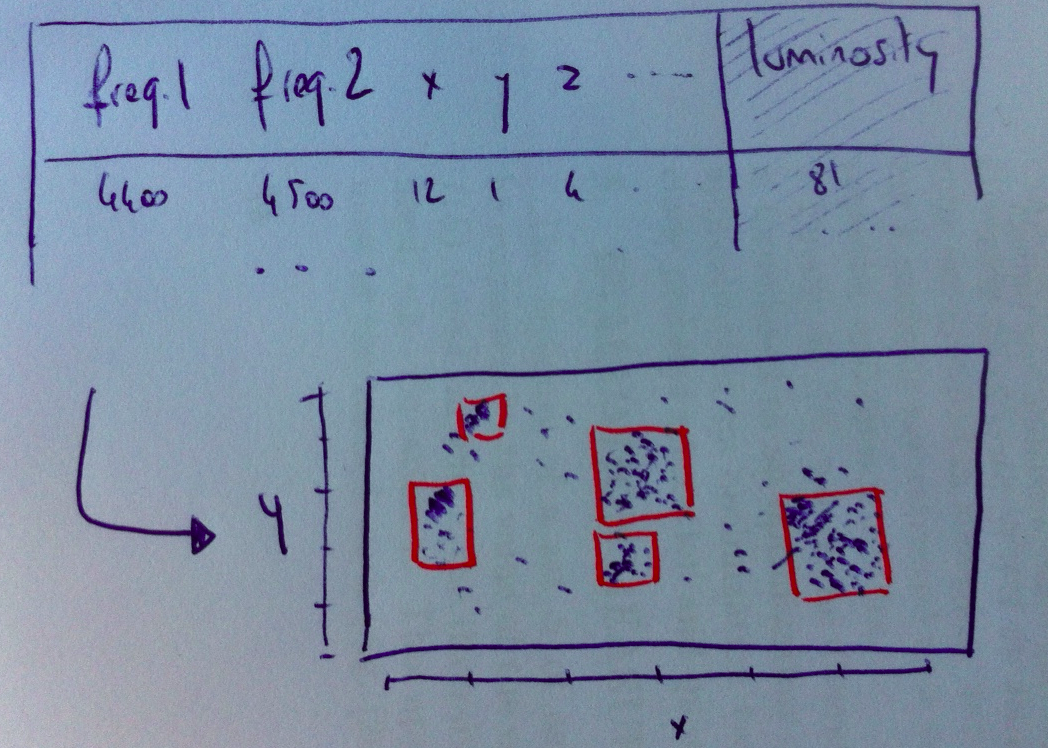
\includegraphics[width=0.8\columnwidth]{images/intro}
\caption{Revealing interesting regions}
\label{intro}
\end{figure}

Recommending queries is fundamentally challenging for two reasons. The first
reason is obvious: how do we define ``interestingness''?  The diversity of
opinions in the litterature is rather depressing:  what is interesting for a
user can be extremely boring for another. The second problem is practical.
Even if we had a universal measure of interest, how could we explore the search
space fast enough to find the interesting queries?

Many autors have proposed query recommenders in the past.  A seminal work was
presented by Sarawagi et al. \cite{sarawagi1998discovery}. According to their
paper, the most interesting queries are the most ``surprising'' ones.
Therefore, they propose to build a (log-linear) model over the data, and
identify the largest deviations. More recently, Dash et
al.\cite{dash2008dynamic} proposed a facet selection method, also based on
surprise. These papers have a trait common: they set a model of
interestingness, and the exploit the particularities of their model to speed up
the computations. Nevertheless, are these interestingness models \emph{really}
intersting?

In this paper, we propose to \emph{abstract interestingness away}. We introduce
Claude, our generic query recommendation system. Claude's model is much simpler
that its predecessors. A user gives one, or several \emph{measures of
interest}. Claude finds the regions with the largest deviations. Claude's
strength comes from its generality: the measure can describe the luminosity of a
star, its deviation from a log-linear model (cf. Sarawagi et al.) or anything
else. Thus, \emph{we let the user decide what is interesting, and we focus on
the search}. Because of the genericity, of our approach, performance is a major
challenge. We introduce two algorithms. The first one is exact, it is based on
level-wise search. The second one is a much faster approximation.
